\newpage
\section{Introduction}
Dans le cadre du développement du système d'information de COPEVUE, il est nécessaire mettre en place une Interface Homme Machine afin de rendre exploitables les différentes données à gérer.
\subsection{Présentation du projet}
COPEVUE souhaite mettre en place un système de monitoring à distance de site isolés. Les différents sites sont répartis dans diverses régions de l'UE et sont pour la plupart difficiles d'accès. Dans le cadre de ce projet, le contrôle des sites consiste en un contrôle de niveau de cuve. COPEVUE souhaite que lorsque le niveau d'une cuve d'un site isolé dépasse un certain seuil critique, ce site envoie un rapport automatiquement au site central qui se chargera de la logistique afin d'envoyer un camion sur le site à ravitailler. Ce projet sera donc utilisé à la fois par des employés au site central, des employés des sociétés de maintenance ou encore directement par les opérateurs de maintenance à l'aide de leur PDAs.

\subsection{Présentation du document}
Ce cahier des charges a pour but de présenter la partie IHM du projet en réponse à l'appel d'offre de COPEVUE, il présentera les problèmes posés et offrira un aperçu de la solution envisagée.
\subsection{Documents des référence}
Une étude préliminaire a déjà été effectuée pour ce projet, pour tout renseignement complémentaire, nous vous encourageons à lire les documents correspondant à l'étude de faisabilité, aux Spécification technique des besoins ainsi que l'analyse de l'existant.

\section{Présentation du problème}
Un des buts recherchés est la possibilité de visualiser en temps réel l'état des différents sites qu'est chargée de contrôler COPEVUE. La solution proposée a donc été conçue en priorité pour traiter ce problème. Le monitoring à distance sous-entend également la possibilité d'effectuer certaines opérations de maintenance à distance sur les systèmes embarqués. L'application développée devra donc être capable de communiquer directement avec les différents sites et de contrôler les systèmes embarqués à distance.

\subsection{But, utilisateurs concernés, nature du logiciel}
Une fois terminé et déployé, ce projet aura pour objectif d'assurer un contrôle complet et en temps réel des différents sites isolés présents en Europe. La première partie se limitera cependant aux sites situés dans le Nord de la Norvège. Le but de ce projet est d'éviter aux propriétaires des sites d'être obligés de contrôler manuellement le niveau des cuves en se rendant sur place. Les données des sites seront directement accessibles à travers l'interface conçue. Les utilisateurs de ce projet seront nombreux et variés, certains se contenteront de consulter des valeurs récupérées des sites isolés, d'autres devront effectuer des rapports de maintenance, d'autres encore devront administrer les systèmes embarqués présents sur les différents sites. \\
Afin de développer une application simple à déployer et à utiliser, nous avons choisi de priviliégier la solution de l'application Web. Cette solution nous permettra de développer une application simple à utiliser, possédant une interface graphique intuitive et très personnalisable en fonction des comptes utilisateurs.

\section{Formulation des besoins, exploitation et ergonomie}
\subsection{Formulation des besoins}
Les besoins exprimés pour ce projet sont simplement la vision et l'exploitation des données reçues des différents sites ainsi que le contrôle à distance des systèmes embarqués situés dans ces sites.

\subsection{exploitation et ergonomie}
La mise en place du projet d'amélioration du système d'information de COPEVUE nécessitera l'installation sur chaque site de divers capteurs permettant de mesurer le niveau de la cuve. Un système embarqué sera également installé afin d'exploiter les données des capteurs et d'envoyer les informations au site central.\\
ce projet aura pour objectif de permettre l'affichage des données recueillies par les capteurs au travers d'une interface simple et intuitive. Elle permettra également de consulter les différents plannings d'intervention sur les sites isolés et la mise à jour de ceux-ci.

\subsection{Portée, développement, mise en œuvre, organisation de la maintenance}
La Solution retenue pour ce projet consiste en une application web. Son développement pourra être effectué par une petite équipe de programmeurs en raison de sa simplicité.\\
Une fois développée, le déploiement de la solution sera immédiat : toute poste de travail ou plateforme mobile disposant d'un accès à internet et d'un navigateur sera en mesure d'y accéder. Il faudra cependant créer les différents comptes utilisateurs permettant aux employés de s'identifier de manière sécurisée afin de pouvoir utiliser l'application. Un gestion des droits est également obligatoire afin que l'application puisse s'adapter au mieux aux différents postes.

\subsection{Limites}
L'application étant uniquement disponible en ligne, il sera impossible d'accéder aux données des sites sans connexion internet : il ne sera pas possible de consulter des données vues précédemment sans connexion internet. 

\section{Exigences fonctionnelles}
\subsection{Fonctions de base, performances et aptitudes}
La fonction principale de cette application sera de permettre un suivi en temps réel de l'état des cuves des différents sites suivis. L'application devra pouvoir afficher de manière claire et rapide les informations concernant les sites.\\
Une fois ces données reçues, le site central devra être en mesure de calculer les itinéraires et d'affecter les différents sites à des plannings à envoyer aux sociétés de maintenance. Finalement, les sociétés de maintenance utiliseront cette application pour visualiser les plannings qui leur ont été affectés et mettre à jour les opérations de maintenance qu'elles ont effectué sur les sites.

\subsection{Contraintes d'utilisation, normes de documentation}
Les principaux utilisateurs de cette IHM étant des non-informaticiens, un soin tout particulier sera apporté au caractère ergonomique de la solution. L'interface devra être simple, claire et facile à utiliser. Un manuel d'utilisateur sera livré lors du déploiement de la solution.

\subsection{Critères d'appréciation}
La principale contrainte d'utilisation étant l'ergonomie, la solution sera en priorité évaluée en fonction de ce critère. Une attention particulière sera cependant apportée à la légèreté de l'application afin de la rendre exploitable par des PDAs dont la vitesse de connexion internet est très dépendante des réseaux disponibles.

\subsection{Flexibilité, variation de coûts associée}
L'application à développer sera accessible à la fois depuis des postes fixes (au site Central) et depuis des PDAs (ceux des camioneurs de l'entreprise de maintenance). Elle devra par conséquent être adaptée en version mobile afin d'être exploitable depuis une plateforme mobile. Le développement d'une version mobile de l'application engendrera un léger surcoût ainsi qu'un temps de développement et de tests plus important.

\section{Contraintes imposées et faisabilité technologique}
\subsection{Sûreté, planning, organisation, communication}
La sécurité des données étant très importante, un soin tout particulier sera apporté à la gestion des comptes utilisateurs afin d'éviter toute corruption de données. La solution développée devra permettre de nombreux accès simultanés aux bases de données ainsi qu'une mise à jour en temps réel des différents tableaux de visualisation des données.

\subsection{Complexité}
La difficulté de développement de cette application n'est pas très élevée : il s'agit principalement d'exploiter des bases de données et d'afficher les résultats.
La principale difficulté lors de la phase de développement résidera dans la vérification constante de la compatibilité de l'application avec les différents navigateurs ainsi que l'ergonomie de la version mobile.

\subsection{Compétences, moyens et règles}
Le développement d'une application web nécessite une bonne connaissance en langages webs et en programmation réseau afin d'être en mesure d'optimiser les performances du produit fini. Le développement de la version mobile demande également certaines compétences spécifiques et une bonne notion des principes de création d'interfaces ergonomiques afin de fournir aux utilisateurs non-informaticiens un système facile à prendre en main.\\
ci dessous, un premier aperçu d'un interface réalisable : \\
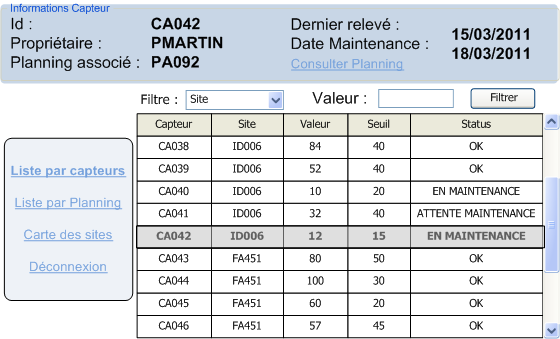
\includegraphics[width=0.9\textwidth]{AppliWebMonitor.png} 

\section{Configuration cible}
\subsection{Matériel et logiciels}
Le matériel sur lequel sera déployée cette application est très variable : du poste de travail fixe au site central au PDA d'un employé de la société de maintenance. Cette grande diversité de matériel cible est cependant compensée par le fait qu'un application web ne dépend pas d'un système en particulier : il suffira en effet de vérifier sa compatibilité avec les différents navigateurs présents sur les plateformes de déploiement. Seule une légère modification de l'application sera effectuée afin d'avoir à disposition une version mobile plus limitée mais plus exploitables sur des PDAs.

\subsection{Stabilité}
La stabilité de l'application est un point clé du projet : les données doivent être récupérées régulièrement afin de satisfaire la contrainte générale de fiabilité du système de monitoring. L'application devra donc être compatible avec les principaux navigateurs disponibles aussi bien sur postes fixes que sur PDAs et de nombreux tests auront pour but d'étudier sa stabilité à long terme.

\subsection{Interfaces}
L'application sera sera principalement en communication avec les bases de données du site central stockant les plannings et informations concernant les sites. Les opérations des mise à jour, et de maintenance à distance la mettront cependant en communication directe avec les systèmes embarqués des sites.

\section{Guide de réponse au cahier des charges}
\subsection{Grille d'évaluation}
	\begin{tabular}{l l l}
	\hline
	Fonction & Priorité & Compléxité \\
	\hline
	Définition des différentes fenêtres & haute & moyenne \\
	Spécification et conception de l'algorithme & haute & faible \\
	Mise en place des outils & haute & faible \\
	
	\hline
            
        \end{tabular}
